\section{Sintesi}
La sintesi schematica della componente si presenta come nella figura sottostante.

\begin{center}
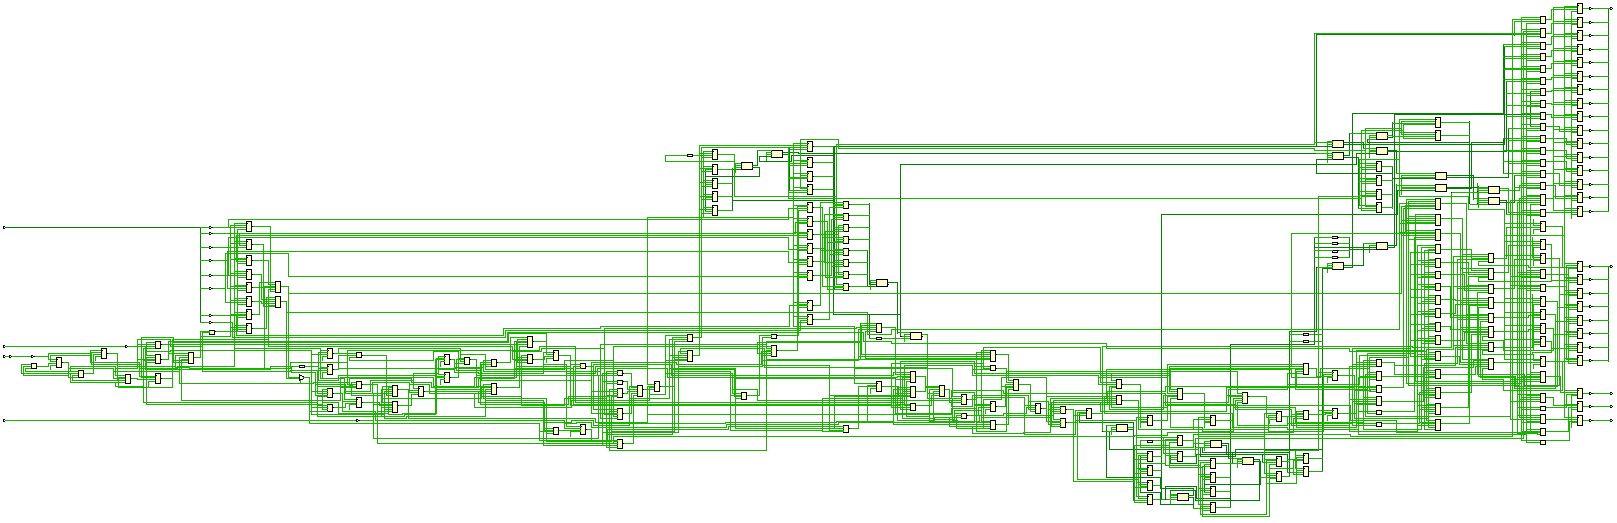
\includegraphics[width=\textwidth]{images/Schematic.png}
\end{center}

\section{Report Utilization}
Segue la tabella che descrive la slice logic della macchina a seguito della sintesi, ottenuta grazie al comando \codeword{report_utilization} fornito da Vivado:

\begin{center}
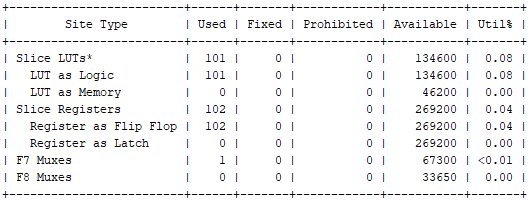
\includegraphics[width=0.8\textwidth]{images/report_uilization.png}
\end{center}

\section{Report Timing}
Da specifica, deve essere progettato un componente che sia funzionante per un tempo di clock $T_{clock}\leq 100 ns$. Il comando \codeword{report_timing_summary} mostra che il Worst Negative Slack (WNS) e il Worst Hold Slack (WHS) sono positivi, quindi il vincolo viene rispettato correttamente. Segue quanto mostrato dal report:

\begin{center}
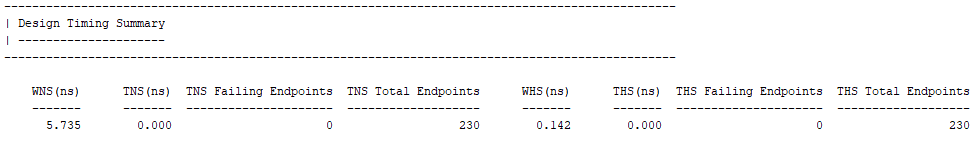
\includegraphics[width=\textwidth]{images/report_timing.png}
\end{center}

\section{Simulazioni}
Il componente progettato è stato testato per verificarne il corretto funzionamento con la sottomissione a testbench randomicamente generati, e ad ulteriori testbench contenenti i casi limite di seguito riportati: 
\begin{itemize}
    \item \textbf{Sequenza Minima}: si testa il caso in cui la parola di memoria in posizione 0000, ossia quella contenente il numero di parole di cui si richiede la lettura, sia nulla. Ci aspettiamo quindi che la convoluzione termini, e che le parole di memoria dalla cella 1000 in poi siano vuote.
    \begin{center}
    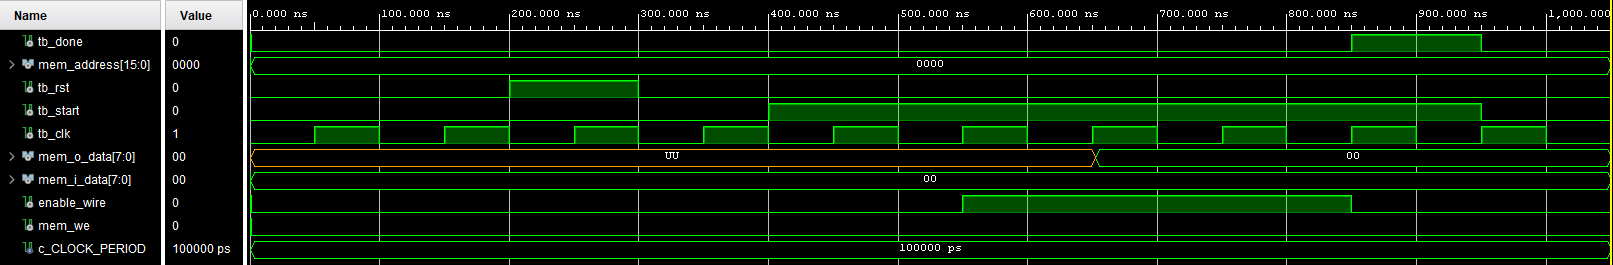
\includegraphics[width=0.93\textwidth]{images/simulations/SeqMin.png}
    \end{center}
    \item \textbf{Sequenza Massima}: si testa il caso in cui la parola di memoria in posizione 0000 contenga il numero di parole massime ricevibili in input (da specifica, 255). Al termine dell’elaborazione, agli indirizzi successivi al 1000, ci aspettiamo siano salvate le parole correttamente codificate.
    \begin{center}
    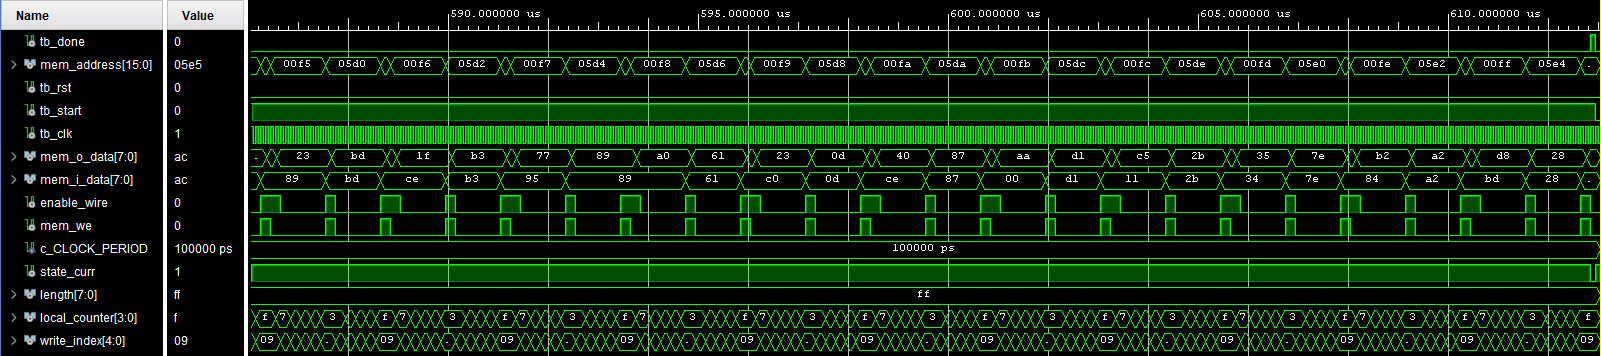
\includegraphics[width=0.93\textwidth]{images/simulations/SeqMax.png}
    \end{center}
    \item \textbf{Reset Improvviso}: il convolutore inizia la lettura della RAM, ma riceve improvvisamente un segnale di reset che riporta la componente nello stato iniziale. Ci aspettiamo che la convoluzione avvenga comunque, e che le parole salvate in memoria siano le stesse che verrebbero salvate in assenza di reset improvviso.
    \begin{center}
    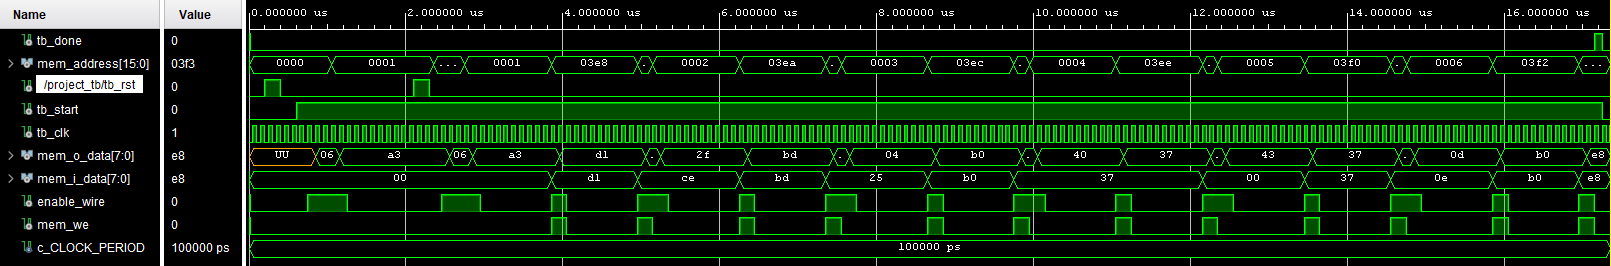
\includegraphics[width=0.93\textwidth]{images/simulations/TBReset.png}
    \end{center}
    \item \textbf{Re-Encode}:  il convolutore viene testato sottoponendolo a tre sequenze diverse di input nella stessa test bench; ci aspettiamo che la codifica avvenga correttamente per tutte e tre le sequenze.
    \begin{center}
    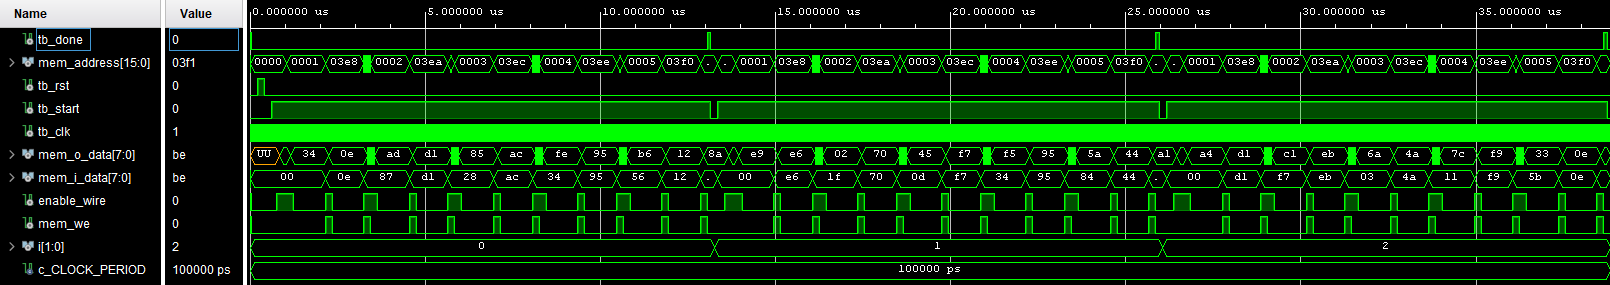
\includegraphics[width=0.93\textwidth]{images/simulations/REEncode.png}
    \end{center}
    \item \textbf{Doppio Uguale}: viene eseguito un double processing. Dopo aver inizializzato la RAM, il testbench procede col verificare che gli output sono stati corretttamente generati dalla macchina e che le parole siano state convolute correttamente. A questo punto, viene inviato un nuovo segnale di \codeword{i_start} in modo tale che la macchina elabori nuovamente le stesse parole studiate in precedenza. Viene quindi verificato che a parità di input, l’output non cambia.
    \begin{center}
    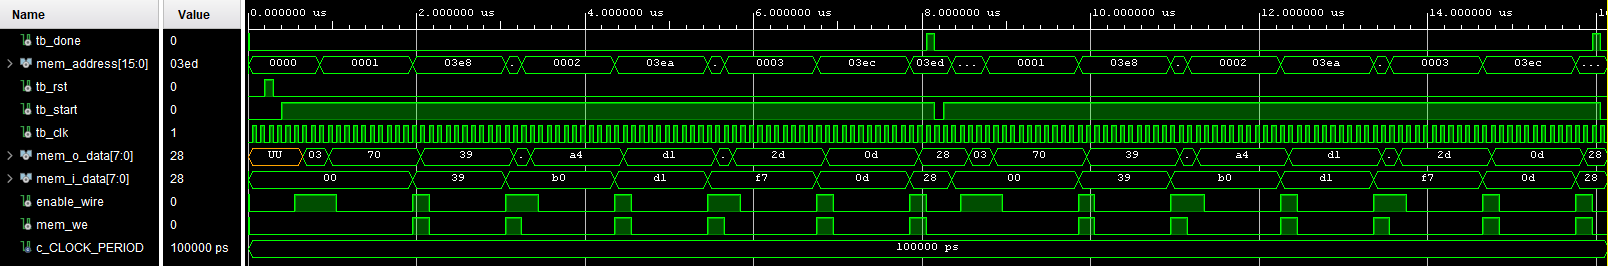
\includegraphics[width=0.93\textwidth]{images/simulations/DoppioUguale.png}
    \end{center}
\end{itemize}
Per verificare il corretto funzionamento, soprattutto in fase di progetto, sono stati utilizzati il testbench fornito dai docenti e altri test prodotti da un generatore casuale.